The primary structure of a protein can be described as a linear sequence of amino acids, also called residues.
They are connected to each other by peptide bonds (Fig. \ref{fig:primary_structure}).
These amide bonds link the $\alpha$-carboxyl group of one amino acid to the amino group of the next.
A polypeptide chain has directionality, 
by convention it start with the amino group and ends with the carboxyl group. 
In the sequence YGGLHAV, Tyrosine (TYR, Y) is the amino-terminal (N-terminal) residue and Valine (VAL, V) the carboxyl-terminal (C-terminal) residue.
The reverse sequence VAHLGGY will have other chemical properties and display other dynamical and conformational behaviour.
Therefore it is considered a different peptide.
The $\alpha$-carbon ($C_{\alpha}$) plus the amino group (NH) and carboxylic acid group (CO) that are connected to it are the same for every residue.
Therefore, a repeating pattern (...-NH-$C_{\alpha}$-CO-NH-...) is observed throughout the sequence.
This constant pattern is called the backbone or mainchain of the protein.
Each residue has also a variable sidechain.
As opposed to DNA,
the backbone of proteins is uncharged.
Therefore, amino acids polymers can form tightly packed globular structures
(\cite{berg2015}).

~\begin{figure}[h!]
	\centering
	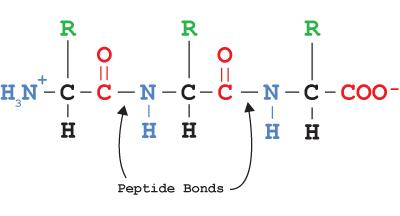
\includegraphics[height=0.25\textheight]{./literature_review/proteins/primary_structure/img/primary_structure.jpg}
	\caption{
		\textbf{The primary structure of a small peptide with three amino acids.}
	(from cbm.msoe.edu).
	}
	\label{fig:primary_structure}
~\end{figure}
